% !TeX encoding = UTF-8

% 载入 SJTUThesis 模版
\documentclass[type=master, lang=zh]{sjtuthesis}
% 选项
%   type=[doctor|master|bachelor],     % 可选(默认:master),论文类型
%   zihao=[-4|5],                      % 可选(默认:-4),正文字号大小
%   lang=[zh|en],                      % 可选(默认:zh),论文的主要语言
%   review,                            % 可选(默认:关闭),盲审模式
%   [twoside|oneside],                 % 可选(默认:twoside),双页或单页边距模式
%   [openright|openany],               % 可选(默认:openright),奇数页或任意页开始新章

% 论文基本配置,加载宏包等全局配置
% !TEX root = ./main.tex

\sjtusetup{
  %
  %******************************
  % 注意:
  %   1. 配置里面不要出现空行
  %   2. 不需要的配置信息可以删除
  %******************************
  %
  % 信息录入
  %
  info = {%
    %
    % 标题
    %
    title           = {基于Bi-LSTM和全局自注意层GRU的中文命名实体识别方法},
    title*          = {A Sample Document for \LaTeX-based SJTU Thesis Template},
    %
    % 标题页标题
    %   可使用“\\”命令手动控制换行
    %
    % display-title   = {上海交通大学学位论文\\ \LaTeX{} 模板示例文档},
    % display-title*  = {A Sample Document \\ for \LaTeX-based SJTU Thesis Template},
    %
    % 关键词
    %
    keywords        = {命名实体识别, 自注意力, Bi-LSTM},
    keywords*       = {SJTU, master thesis, XeTeX/LaTeX template},
    %
    % 姓名
    %
    author          = {陈\quad{}朝},
    author*         = {Mo Mo},
    %
    % 指导教师
    %
    supervisor      = {韩东教授},
    supervisor*     = {Prof. Dong Han},
    %
    % 副指导教师
    %
    % assoc-supervisor  = {某某教授},
    % assoc-supervisor* = {Prof. Uom Uom},
    %
    % 学号
    %
    id              = {121071910003},
    %
    % 学位
    %   本科生不需要填写
    %
    degree          = {应用统计专业硕士},
    degree*         = {Master of Applied Statistics},
    %
    % 专业
    %
    major           = {应用统计},
    major*          = {Applied Statistics},
    %
    % 所属院系
    %
    department      = {数学科学学院},
    department*     = {School of Mathematical Sciences},
    %
    % 答辩日期
    %   使用 ISO 格式 (yyyy-mm-dd);默认为当前时间
    %
    % date            = {2014-12-17},
    %
    % 资助基金
    %
    % fund  = {
    %           {国家 973 项目 (No. 2025CB000000)},
    %           {国家自然科学基金 (No. 81120250000)},
    %         },
    % fund* = {
    %           {National Basic Research Program of China (Grant No. 2025CB000000)},
    %           {National Natural Science Foundation of China (Grant No. 81120250000)},
    %         },
  },
  %
  % 风格设置
  %
  style = {%
    %
    % 论文标题页 logo 颜色 (red/blue/black)
    %
    % title-logo-color = black,
  },
  %
  % 名称设置
  %
  name = {
    % bib             = {References},
    % ack             = {谢\hspace{\ccwd}辞},
    % achv            = {攻读学位期间完成的论文},
  },
}

% 使用 BibLaTeX 处理参考文献
%   biblatex-gb7714-2015 常用选项
%     gbnamefmt=lowercase     姓名大小写由输入信息确定
%     gbpub=false             禁用出版信息缺失处理
\usepackage[backend=biber,style=gb7714-2015]{biblatex}
% 文献表字体
% \renewcommand{\bibfont}{\zihao{-5}}
% 文献表条目间的间距
\setlength{\bibitemsep}{0pt}
% 导入参考文献数据库
\addbibresource{bibdata/thesis.bib}

% 脚注格式
\usepackage[perpage,bottom,hang]{footmisc}

% 定义图片文件目录与扩展名
\graphicspath{{figures/}}
\DeclareGraphicsExtensions{.pdf,.eps,.png,.jpg,.jpeg}

% 确定浮动对象的位置,可以使用 [H],强制将浮动对象放到这里(可能效果很差)
% \usepackage{float}

% 固定宽度的表格
% \usepackage{tabularx}

% 使用三线表:toprule,midrule,bottomrule。
\usepackage{booktabs}

% 表格中支持跨行
\usepackage{multirow}

% 表格中数字按小数点对齐
\usepackage{dcolumn}
\newcolumntype{d}[1]{D{.}{.}{#1}}

% 使用长表格
\usepackage{longtable}

% 附带脚注的表格
\usepackage{threeparttable}

% 附带脚注的长表格
\usepackage{threeparttablex}

% 算法环境宏包
\usepackage[ruled,vlined,linesnumbered]{algorithm2e}
% \usepackage{algorithm, algorithmicx, algpseudocode}

% 代码环境宏包
\usepackage{listings}
\lstnewenvironment{codeblock}[1][]%
  {\lstset{style=lstStyleCode,#1}}{}

% 物理科学和技术中使用的数学符号,定义了 \qty 命令,与 siunitx 3.0 有冲突
% \usepackage{physics}

% 直立体数学符号
\providecommand{\dd}{\mathop{}\!\mathrm{d}}
\providecommand{\ee}{\mathrm{e}}
\providecommand{\ii}{\mathrm{i}}
\providecommand{\jj}{\mathrm{j}}

% 国际单位制宏包
\usepackage{siunitx}[=v2]

% 定理环境宏包
\usepackage{ntheorem}
\usepackage{cases}
\usepackage{amsmath}
% \usepackage{amsthm}

% 绘图宏包
\usepackage{tikz}
\usetikzlibrary{shapes.geometric, arrows}

% 一些文档中用到的 logo
\usepackage{hologo}
\providecommand{\XeTeX}{\hologo{XeTeX}}
\providecommand{\BibLaTeX}{\textsc{Bib}\LaTeX}

% 借用 ltxdoc 里面的几个命令方便写文档
\DeclareRobustCommand\cs[1]{\texttt{\char`\\#1}}
\providecommand\pkg[1]{{\sffamily#1}}

% 自定义命令

% E-mail
\newcommand{\email}[1]{\href{mailto:#1}{\texttt{#1}}}

% hyperref 宏包在最后调用
\usepackage{hyperref}

% 自动引用题注更正为中文
\def\equationautorefname{式}
\def\footnoteautorefname{脚注}
\def\itemautorefname{项}
\def\figureautorefname{图}
\def\tableautorefname{表}
\def\partautorefname{篇}
\def\appendixautorefname{附录}
\def\chapterautorefname{章}
\def\sectionautorefname{节}
\def\subsectionautorefname{小节}
\def\subsubsectionautorefname{小节}
\def\paragraphautorefname{段落}
\def\subparagraphautorefname{子段落}
\def\FancyVerbLineautorefname{行}
\def\theoremautorefname{定理}


\begin{document}

%TC:ignore

% 标题页
\maketitle

% 原创性声明及使用授权书
\copyrightpage
% 插入外置原创性声明及使用授权书
% 此时必须在导言区使用 \usepackage{pdfpages}
% \copyrightpage[scans/sample-copyright-old.pdf]

% 前置部分
\frontmatter

% 摘要
\input{contents/abstract}

% 目录
\tableofcontents
% % 插图索引
% \listoffigures*
% % 表格索引
% \listoftables*
% % 算法索引
% \listofalgorithms*

% % 符号对照表
% \input{contents/nomenclature}

%TC:endignore

% 主体部分
\mainmatter

% 正文内容
% !TEX root = ../main.tex

\chapter{绪论}


\section{研究背景与意义}

命名实体识别指的是从文本中识别出重要对象(例如人,组织,地点)的自然语言处理任务\parencite{erdogan2010sequence}。
后面我们将使用NER来指代命名实体识别和分类。NER是信息提取、问答系统、句法分析、机器翻译、
面向语义网的元数据标注等应用领域的重要基础工具,在自然语言处理技术走向实用
化的过程中占有重要地位。

NER任务通常包括两部分:(1)实体边界识别;(2)确定实体类别(人名、地名、机构名或其他)。
英语中的命名实体具有比较明显的形式标志(即实体中的每个词的第一个字母要大写),所以实体边界
识别相对容易,任务的重点是确定实体的类别。和英语相比,汉语命名实体识别任务更加复杂,而且相
对于实体类别标注子任务,实体边界的识别更加困难。


\section{国内外研究进展}


\subsection{基于规则的命名实体识别方法}

基于规则和字典的方法是最初代的命名实体识别使用的方法,这些方法多采用由语言学家通过人工方式,
依据数据集特征构建的特定规则模板或者特殊词典。规则包括关键词、位置词、方位词、中心词、指示词、
统计信息、标点符号等。词典是由特征词构成的词典和外部词典共同组成,外部词典指已有的常识词典。
制定好规则和词典后,通常使用匹配的方式对文本进行处理以实现命名实体识别。

这种方法所训练出来的模型通常过拟合于非常特定的结构化文本语料库,如军事信息集、海军作战报告、并购新闻等。


\subsection{基于统计的命名实体识别方法}

\subsubsection{监督学习方法}

在大型注释语料库上训练的监督学习技术为NER提供了当时最好的结果。著名的监督学习算法
主要包括隐马尔可夫模型(HMM)、决策树、最大熵模型(ME)、支持向量机(SVM)、条件随机场(CRF)。
特别是CRF算法是最有效的NER算法之一。NER需要使用许多前导和滞后的非局部序列训练输出标签的概率,
这使得像CRF这样的判别模型比生成模型更为适合。尽管ME模型放宽了生成模型所做的强独立性假设,但他们存在标签偏差问题,
即模型偏向于输出过渡较少的状态。CRF通过联合考虑所有状态中不同特征的权重来解决这一问题,而不是将状态级别的转移概率归一化。
\parencite{sarawagi2004semi}通过制定半CRF模型改进了现有CRF模型,该模型将标签分配给子序列而不是单个实体,并且没有任何显著的额外计算复杂度。
\parencite{passos2014lexicon}在公共数据上使用他们的词典注入Skip-gram模型来学习高质量的短语向量,并将其插入对数线性CRF系统。
实体分析的联合模型(多任务模型)在单个任务上的结果比单独为NER优化的模型更好。
\parencite{durrett2014joint}开发了一个结构化的CRF模型,该模型通过训练3个任务来提高NER(以及其他实体分析任务)的性能,
例如共指解析(文档内聚类)、命名实体识别(粗语义类型)和实体链接(匹配维基百科实体)。



\subsubsection{半监督学习方法}

\parencite{luo2015joint}提出了JERL(Joint Entity Recognition and Linking)模型,即扩展半CRF模型以捕获NER和实体链接之间的依赖关系。
监督学习方法遇到了障碍,因为可用于学习判别特征的结构化文本是有限的。这催生了半监督学习方法,
它利用了非结构化文本的指数增长量,换句话说,网页以无监督的方式从种子注释语料库中获取上下文信息,即bootstarpping。
\parencite{luo2015joint}提出了一种无监督方法,从大规模未标记数据中创建资源丰富的浓缩特征表示,以有效地训练有监督的NER系统,同时仍保持现有高维半监督解决方案的最新结果。



\subsubsection{无监督学习方法}

无监督学习方法主要是从作为输入词的上下文中生成附加特征以与其他 NER 方法结合使用的手段。
\parencite{lin2009phrase}通过在搜索引擎查询日志的私有数据库上执行 K-means 聚类以使用聚类特征来训练他们的CRF模型,
从而在不使用地名词典的情况下获得了当时最优的结果。无监督学习技术工业应用的一个例外是使用词汇资源的聚类方法,
例如Wordnet以便从Wordnet本身分配命名实体类型。尽管为此目的广泛采用了CRF,但仍有许多关于使用神经网络进行NER的论文。
\parencite{ratinov2009design}在感知机模型中使用了非局部特征、从维基百科中提取的地名词典和类似布朗簇的词表示。由于多层前馈神经网络是通用逼近器,
因此这种神经网络也可以潜在地解决NER任务。


\subsection{基于深度学习的命名实体识别方法}

\subsubsection{卷积神经网络}

卷积神经网络(CNN)可以使用反向传播学习丛单词中提取特征向量表示。因此,在从可变长度的输入序列中提取高阶特征时,
CNN似乎是自然选择。有两种方法:(1)窗口法和(2)(卷积)句法。窗口方法假设分配给单个单词的标签取决于它的上下文
(即出现在给定单词之前或之后的单词),该方法更适合于像NER这样的序列标记任务。

\begin{equation}
	f^{l}_{\theta}
	= \langle LT_W( [ w ] ^T_l) \rangle ^{d_{win}}_t
	= \left(
			\begin{array}{c}
			\langle W \rangle ^l_{[w]_{t - d_{win} / 2}} \\
			\vdots \\
			\langle W \rangle ^l_{[w]_t} \\
			\vdots \\
			\langle W \rangle ^l_{[w]_{t + d_{win} / 2}}
		\end{array} 
	\right)
\end{equation}


\begin{equation}
	f^{l}_{\theta} 
	= W^l f^{l - 1}_{\theta} + b^l
\end{equation}

这里的$W^l \in R^{ n^l_h \times n^{l - 1}_h}$和$b^l \in R^{n^l_h}$是使用反向传播训练的,
$n^l_h$是一个超参数,表示该层中隐藏单元的数量。固定大小的矢量输入可以通过如上所示的多个线性变换层进行传递。
为了从输入序列中捕获高阶特征,存在“硬”双曲正切函数层。“硬”双曲正切在防止过拟合的同时,与精确双曲正切函数相比,
计算效率更高。窗口特性的一个警告是,句首和句尾单词的上下文没有明确定义。因此,在输入句子的开头和结尾都有相当于
窗口一半大小的填充词,类似于序列模型中的开始和停止指示器。


\begin{equation}
	[f^{l}_{\theta}]_i 
	= Hard tanh([f^{l - 1}_{\theta}]_i)
\end{equation}


\begin{equation}
	Hard tanh(x)
    = \begin{cases}
        -1 & x < -1 \\
        x & -1 \geq x \leq 1 \\
        1 & x \geq 1
    \end{cases}
\end{equation}


使用CNN进行句子建模可以追溯到\parencite{collobert2008unified}。该工作使用多任务学习来输出对NLP任务的多个预测,
如POS标记、块、命名实体标记、语义角色、语义相似词和一个语言模型。使用一个查找表将每个单词转换为用户定义的维度向量。
因此,通过对每个单词应用查找表,n个单词的输入序列$s_1,s_2,\cdots, s_n$被转换为一系列向量$ws_1,ws_2, \cdots, ws_n$。


这可以看作是一种原始词嵌入方法,其权值是在网络训练中习得的。在\parencite{collobert2011natural}中,Collobert扩展了他们的工作,
提出了一个通用的基于CNN的框架来解决过多的NLP任务。这两篇文章使得CNN在自然语言处理研究人员中得到了广泛普及。
鉴于CNN在计算机视觉任务上已经展现出了它们的实力,人们更容易相信它们的表现。
CNN能够从输入句子中提取显著的N-gram特征,为下游任务创建句子的信息潜在语义表示。
这样的应用是由\parencite{collobert2011natural, kim2016character, kalchbrenner2014convolutional}初创的,这催生了后续文献中以CNN为基础的网络的大量扩散。

\subsubsection{循环神经网络}


循环神经网络是深度神经网络体系结构的另一种形式。一般来说,CNN被用来表示位置不变的函数(如词袋),
而RNN则表示顺序的体系结构(如句子、段落等)。很明显,相对于分层CNN, RNN更适合于像NER这样的序列建模任务。
虽然我们看到窗口方法有助于处理CNN中的序列输入,但除了在交叉验证中固定的之外,没有办法对上下文依赖性建模。
RNN帮助捕捉单词或句子的依赖性,这超出了CNN的固定范围。简单的RNN没有门控机制。RNN是一种跨时间展开的网络,
因此提供了记忆的空间表示。对于一个给定的输入,RNN计算一个隐藏状态如下:

\begin{equation}
	[s^t_{\theta, l}]_i = g_{\theta, l}([f^t_{\theta, l}]_i)
\end{equation}

\begin{equation}
	[f^t_{\theta, l}]_i = W^l[x^t_l]_i + [s^{t-1}_{\theta, l}]_i
\end{equation}

这里$[s^t_{\theta, l}]_i$是输入序列的单位在$t$时刻和$l$层的隐藏状态。
$g_{\theta, l}$是在以$[f^t_{\theta, l}]_i$为输入层上的一个非线性函数(如$tanh$等)。
$x^t_l$是在$t$时刻和通过训练得到的权重$W^l \in R^{d_{s^{t}_{\theta, l}} \times d_{x^t_l}}$上输入序列的第$i$个单元(单词,句子等)。
简单RNN中的隐藏状态可以看作是它的记忆分量。然而,简单RNN存在梯度消失的问题,这使得反向传播很难学习到之前的权值。
因此,简单RNN增加了门控机制来克服收敛问题。具有门控机制的RNN变体在神经网络中最受欢迎的是长短期记忆网络(LSTM)和门控循环单元(GRUs)。


\paragraph{长短期记忆网络}

LSTM\parencite{graves2012long}的新奇之处在于它能够跨越长时间间隔(快速学习许多时间步后缓慢变化的权值,如长期记忆)
以及保存最近的输入(例如短期记忆)。此外,LSTM架构确保了不断的重新加权,从而避免了通过隐藏状态错误流的爆发或消失。

\begin{numcases}{}
	i_t = \sigma(x_t U^i + h_{t-1} W^i + b_i) \\
	f_t = \sigma(x_t U^f + h_{t-1} W^f + b_f) \\
	o_t = \sigma(x_t U^o + h_{t-1} W^o + b_o) \\
	q_t = tanh(x_t U^q + h_{t-1} W^q + b_q) \\
	p_t = f_t \times p_{t-1} + i_t \times q_t \\
	h_t = o_t \times tanh(p_t)
\end{numcases}

LSTM有三个门:输入门$i_t$、遗忘门$f_t$和输出门$o_t$,它们是$Sigmoid$函数在输入$x_t$和前面的隐藏状态$h_{t-1}$上的输出。
为了生成当前第$t$步的隐藏状态,它首先通过在输入$x_t$和之前的隐藏状态$h_{t-1}$上运行非线性$tanh$函数生成一个临时变量$q_t$。
然后LSTM计算一个在时刻$t$更新的历史变量$p_t$作为前一个历史状态$p_{t-1}$和当前临时变量$q_t$的线性组合,
分别由当前遗忘门$f_t$和当前输入门$o_t$。最后,LSTM运行$tanh$,并根据当前输出门对其进行缩放,以获得更新后的隐藏状态。

虽然LSTM善于近似序列的当前单元与前一个单元的相关性,但它没有考虑到当前单元与序列中其右侧单元的相关性。
\parencite{lample2016neural}通过实现双向LSTM解决了这个问题\parencite{graves2005framewise}。
换句话说,有两个独立的LSTM,分别使用目标词的左侧和右侧的输入序列片段进行训练。
该模型通过分别连接前向和后向LSTM的左右上下文表示,即隐藏状态$h_t = [h_t^{\rightarrow};h_t^{\leftarrow} ]$,获得目标词的完整表示。


\paragraph{门控循环单元}

与LSTM相比,门控循环单元[57]是一种较新的、较不复杂的RNN变体。

GRU与LSTM相似,因为它可以调节错误流,从而避免梯度消失\parencite{bengio1994learning}。然而,GRU与LSTM有许多关键的区别。
GRN不像LSTM那样有独立的存储单元。因此,GRN缺乏对内存内容(即LSTM的输出门)的受控外显。
与LSTM不同,GRN在没有任何控制的情况下公开完整的内容。此外,GRN控制着从前一个激活状态到当前候选激活状态的信息流。
另一方面,LSTM在不控制历史信息流的情况下计算最新的内存内容。GRU的工作原理如下:

\begin{numcases}{}
	h^j_t = (1 - z^j_t)h^j_{t-1} + z^j_t \overline{h}^j_t \\
	z^j_t = \sigma(W_z x_t + U_z h_{t-1}) \\
	\overline{h}^j_t = tanh(Wx_t + U(r_t \odot h_{t-1})) \\
	r^j_t = \sigma(W_r x_t + U_r h_{t-1})
\end{numcases}


$h^j_t$是GRU在时刻$t$时第$j$级的激活状态。$\overline{h}^j_t$是GRU在时刻$t$时第$j$级的候选激活状态\parencite{bahdanau2014neural}。
更新门$z^j_t$决定了单元更新其激活状态的程度。重置门$r^j_t$的计算方法与更新门类似。


\section{论文组织结构}


% 上海交通大学是我国历史最悠久的高等学府之一,是教育部直属、教育部与上海市共建的全
% 国重点大学,是国家“七五”、“八五”重点建设和“211 工程”、“985 工程”的首批建
% 设高校。经过 115 年的不懈努力,上海交通大学已经成为一所“综合性、研究型、国际化”
% 的国内一流、国际知名大学,并正在向世界一流大学稳步迈进。 

% {\songti 十九世纪末,甲午战败,民族危难。中国近代著名实业家、教育家盛宣怀和一批
%   有识之士秉持“自强首在储才,储才必先兴学”的信念,于 1896 年在上海创办了交通大
%   学的前身——南洋公学。建校伊始,学校即坚持“求实学,务实业”的宗旨,以培养“第
%   一等人才”为教育目标,精勤进取,笃行不倦,在二十世纪二三十年代已成为国内著名的
%   高等学府,被誉为“东方MIT”。抗战时期,广大师生历尽艰难,移转租界,内迁重庆,
%   坚持办学,不少学生投笔从戎,浴血沙场。解放前夕,广大师生积极投身民主革命,学校
%   被誉为“民主堡垒”。
  
%   新中国成立初期,为配合国家经济建设的需要,学校调整出相当一部分优势专业、师资设
%   备,支持国内兄弟院校的发展。五十年代中期,学校又响应国家建设大西北的号召,根据
%   国务院决定,部分迁往西安,分为交通大学上海部分和西安部分。1959 年 3月两部分同
%   时被列为全国重点大学,7 月经国务院批准分别独立建制,交通大学上海部分启用“上海
%   交通大学”校名。历经西迁、两地办学、独立办学等变迁,为构建新中国的高等教育体
%   系,促进社会主义建设做出了重要贡献。六七十年代,学校先后归属国防科工委和六机部
%   领导,积极投身国防人才培养和国防科研,为“两弹一星”和国防现代化做出了巨大贡
%   献。}

% {\heiti 改革开放以来,学校以“敢为天下先”的精神,大胆推进改革:率先组成教授代
%   表团访问美国,率先实行校内管理体制改革,率先接受海外友人巨资捐赠等,有力地推动
%   了学校的教学科研改革。1984 年,邓小平同志亲切接见了学校领导和师生代表,对学校
%   的各项改革给予了充分肯定。在国家和上海市的大力支持下,学校以“上水平、创一流”
%   为目标,以学科建设为龙头,先后恢复和兴建了理科、管理学科、生命学科、法学和人文
%   学科等。1999 年,上海农学院并入;2005 年,与上海第二医科大学强强合并。至此,学
%   校完成了综合性大学的学科布局。近年来,通过国家“985 工程”和“211 工程”的建
%   设,学校高层次人才日渐汇聚,科研实力快速提升,实现了向研究型大学的转变。与此同
%   时,学校通过与美国密西根大学等世界一流大学的合作办学,实施国际化战略取得重要突
%   破。1985 年开始闵行校区建设,历经 20 多年,已基本建设成设施完善,环境优美的现
%   代化大学校园,并已完成了办学重心向闵行校区的转移。学校现有徐汇、闵行、法华、七
%   宝和重庆南路(卢湾)5 个校区,总占地面积 4840 亩。通过一系列的改革和建设,学校
%   的各项办学指标大幅度上升,实现了跨越式发展,整体实力显著增强,为建设世界一流大
%   学奠定了坚实的基础。}

% {\ifcsname fangsong\endcsname\fangsong\else[无 \cs{fangsong} 字体。]\fi 交通大学
%   始终把人才培养作为办学的根本任务。一百多年来,学校为国家和社会培养了 20余万各
%   类优秀人才,包括一批杰出的政治家、科学家、社会活动家、实业家、工程技术专家和医
%   学专家,如江泽民、陆定一、丁关根、汪道涵、钱学森、吴文俊、徐光宪、张光斗、黄炎
%   培、邵力子、李叔同、蔡锷、邹韬奋、陈敏章、王振义、陈竺等。在中国科学院、中国工
%   程院院士中,有 200 余位交大校友;在国家 23 位“两弹一星”功臣中,有 6 位交大校
%   友;在 18 位国家最高科学技术奖获得者中,有 3 位来自交大。交大创造了中国近现代
%   发展史上的诸多“第一”:中国最早的内燃机、最早的电机、最早的中文打字机等;新中国
%   第一艘万吨轮、第一艘核潜艇、第一艘气垫船、第一艘水翼艇、自主设计的第一代战斗
%   机、第一枚运载火箭、第一颗人造卫星、第一例心脏二尖瓣分离术、第一例成功移植同种
%   原位肝手术、第一例成功抢救大面积烧伤病人手术等,都凝聚着交大师生和校友的心血智
%   慧。改革开放以来,一批年轻的校友已在世界各地、各行各业崭露头角。}

% {\ifcsname kaishu\endcsname\kaishu\else[无 \cs{kaishu} 字体。]\fi 截至 2011 年 12
%   月 31 日,学校共有 24 个学院 / 直属系(另有继续教育学院、技术学院和国际教育学
%   院),19 个直属单位,12 家附属医院,全日制本科生 16802 人、研究生24495 人(其
%   中博士研究生 5059 人);有专任教师 2979 名,其中教授 835 名;中国科学院院士 15
%   名,中国工程院院士 20 名,中组部“千人计划”49 名,“长江学者”95 名,国家杰出
%   青年基金获得者 80 名,国家重点基础研究发展计划(973 计划)首席科学家 24名,国
%   家重大科学研究计划首席科学家 9名,国家基金委创新研究群体 6 个,教育部创新团队
%   17 个。
  
%   学校现有本科专业 68 个,涵盖经济学、法学、文学、理学、工学、农学、医学、管理学
%   和艺术等九个学科门类;拥有国家级教学及人才培养基地 7 个,国家级校外实践教育基
%   地 5个,国家级实验教学示范中心 5 个,上海市实验教学示范中心 4 个;有国家级教学
%   团队 8个,上海市教学团队 15 个;有国家级教学名师 7 人,上海市教学名师 35 人;
%   有国家级精品课程 46 门,上海市精品课程 117 门;有国家级双语示范课程 7
%   门;2001、2005 和2009 年,作为第一完成单位,共获得国家级教学成果 37 项、上海市
%   教学成果 157项。}
% !TEX root = ../main.tex


\chapter{基于词嵌入的命名实体识别方案}

\section{嵌入方案介绍}

自然语言处理任务中的一个关键问题就是如何用数学语言去表示自然语言,并且其表示的优劣则会直接影响其下游任务结果的好坏。

\subsection{词嵌入(Word Embedding)}

\paragraph{One-Hot编码}
最简单且最容易实现的的表示方法之一就是给词编码。假如能够列出所有可能出现的词,我们只需要给每个词一个唯一的编码,
即可完成简单的词表示。例如一个词表中有12个词,按照拼音首字母排列如下:

\begin{table}[!hpt]
    \caption[示例词典编码对照表]{示例词典编码对照表}
    \label{tab:case_lookup_table}
    \centering
    \begin{tabular}{lr} \toprule
      词语  &   编码 \\ \midrule
      处理  &   1 \\
      的    &   2 \\
      方案  &   3 \\
      非常  &   4 \\
      命名  &   5 \\
      难以  &   6 \\
      识别  &   7 \\
      实体  &   8 \\
      是    &   9 \\
      学习  &   10 \\
      语言  &   11 \\
      自然  &   12 \\ \bottomrule
    \end{tabular}
\end{table}

“自然语言处理非常难以学习”这句话分词后的结果为(自然, 语言, 处理, 非常, 难以, 学习)用
表~\ref{tab:case_lookup_table}的编码表示就是:(12, 11, 1, 4, 6, 10)。

在使用机器学习算法做自然语言处理任务的时候,模型所接受的输入一般是定长的向量,
所以需要将上表中的所有编码转换为向量。One-Hot编码是使用与词表等长的向量来表示特定词语,向量中的元素只包含0或1。
每个词只有在它对应的位置上元素为1,其余都为0。对于表~\ref{tab:case_lookup_table},
其对应的One-Hot向量如表~\ref{tab:case_one_hot_lookup_table}

\begin{table}[!hpt]
    \caption[示例词典One-Hot向量对照表]{示例词典One-Hot向量对照表}
    \label{tab:case_one_hot_lookup_table}
    \centering
    \begin{tabular}{lrl} \toprule
      词语  &   编码 &  One-Hot向量 \\ \midrule
      处理	&	1	&   [1, 0, 0, 0, 0, 0, 0, 0, 0, 0, 0, 0]	\\
      的	&	2	&	[0, 1, 0, 0, 0, 0, 0, 0, 0, 0, 0, 0]	\\
      方案	&	3	&	[0, 0, 1, 0, 0, 0, 0, 0, 0, 0, 0, 0]	\\
      非常	&	4	&	[0, 0, 0, 1, 0, 0, 0, 0, 0, 0, 0, 0]	\\
      命名	&	5	&	[0, 0, 0, 0, 1, 0, 0, 0, 0, 0, 0, 0]	\\
      难以	&	6	&	[0, 0, 0, 0, 0, 1, 0, 0, 0, 0, 0, 0]	\\
      识别	&	7	&	[0, 0, 0, 0, 0, 0, 1, 0, 0, 0, 0, 0]	\\
      实体	&	8	&	[0, 0, 0, 0, 0, 0, 0, 1, 0, 0, 0, 0]	\\
      是	&	9	&	[0, 0, 0, 0, 0, 0, 0, 0, 1, 0, 0, 0]	\\
      学习	&	10	&	[0, 0, 0, 0, 0, 0, 0, 0, 0, 1, 0, 0]	\\
      语言	&	11	&	[0, 0, 0, 0, 0, 0, 0, 0, 0, 0, 1, 0]	\\
      自然	&	12	&	[0, 0, 0, 0, 0, 0, 0, 0, 0, 0, 0, 1]	\\ \bottomrule
    \end{tabular}
\end{table}

这样表示虽然清晰,但却存在两个严重的问题:
\begin{enumerate}
    \item \textbf{向量维度过高并且高度稀疏}:自然语言处理任务中的词汇量一般非常大。
    例如中文或者英文的常用词有上万个,其他语言也类似。如此多的词语会导致One-Hot向量的维度非常大,
    计算时不仅浪费内存,计算量也极大。
    \item \textbf{信息量少,无法表征语义相似度}:自然语言的词与词之间可能存在一定的关系。
    如果我们用词向量的余弦相似度来衡量两个词的相关性,越接近1或者-1表示两个词语义越相近或者相反,
    越接近0表示语义约不相关。例如“漂亮”和“美丽”是一对近义词,它们的余弦相似度应该接近于1;
    “美丽”和“丑陋”是一对反义词,它们的余弦相似度应该接近于-1;而“美丽”和“手机”在语义上的关系较弱,
    其余弦相似度则应该接近于0。
\end{enumerate}


\paragraph{Word2Vec}

Word2Vec即word to vector,顾名思义就是将词转换为向量。该方法由\parencite{mikolov2013efficient}首创,
主要有以下特点:
\begin{enumerate}
    \item \textbf{算法效率高}:可以在百万数量级的词典和上亿规模的数据上训练;
    \item \textbf{可以表征语义相似度}:得到的词向量可以较好地反应词间的语义关系。
\end{enumerate}

Word2Vec提出了两种基本模型:CBOW(连续词袋模型)和Skip-Gram(跳词模型),来构建单词的高细粒度的向量表示。

\subparagraph{CBOW}
CBOW即Continuous Bag-Of-Words,是通过一个词的上下文来预测这个词的语义。


\subparagraph{Skip-Gram}
Skip-Gram是通过一个词语来预测上下文的词语,其思路正好与CBOW相反。


使用预训练的词嵌入已经成为包括NER在内的NLP任务的标准特征。\parencite{collobert2011natural}提出了一种构建词嵌入的神经网络体系结构,
该体系结构构成了获取词向量表示的主要方法,用于训练NER的深度学习NLP模型。
词嵌入是由\parencite{mikolov2013efficient}首创的,他引入了连续词袋和Skip-gram模型来构建单词的高细粒度的向量表示。
\parencite{pennington2014glove}的Glove是另一种著名的基于词共现的词嵌入方法。通过将矩阵归一化和平滑后的重构损耗最小化,
将频率矩阵分解到较低的维数。[13]创建单词嵌入的方法被广泛采用,因为这种向量表示显示了组合性。
构成性与线性语义推理脑电信号的性质相对应,例如'Paris' - 'France' + 'Italy' = 'Rome'。

CBOW和连续Skip-gram都是对数线性语言模型,但它们在基本种类上有所不同。CBOW根据上下文预测目标词。
然而,连续Skip-gram模型预测给定窗口内目标词前后的单词。用作向量表示上下文的相邻单词窗口是一个需要优化的超参数。
增加窗口增加了语言模型的准确性,但也增加了考虑窗口中较远单词的计算复杂性。

\subsection{字符嵌入(Character Embedding)}

字符级嵌入在NER中被用来捕获跨语言的形态特征。在某些NLP任务中,其对形态丰富的语言有较好的结果。
\parencite{santos2015boosting}NER应用了字符级表示以及单词嵌入,在葡萄牙语和西班牙语语料库中取得了最先进的结果。
\parencite{kim2016character}研究出了仅使用字符嵌入构建神经语言模型的正向结果。\parencite{ma2016end}利用了几种嵌入方法,包括字符三元图,
将原型信息和分层信息结合起来,用于学习NER环境中预训练的标签嵌入。中文是另一种形态学丰富的语言,
在深度学习序列标记模型中,字符嵌入比单词嵌入能表现出更好的性能\parencite{zheng2013deep}。

单词嵌入不传递字符嵌入提供的语义和其他内部信息。因此,字符嵌入能够通过将未知词的含义映射到构成字符或子词的含义来推断未知词的含义。
于是,字符嵌入解决了词汇表外(OOV)词的识别问题,如用于词性标注和语言建模或依赖性解析\parencite{ballesteros2015improved}等任务的输入语料库中不存在的单词。
字符嵌入为表示单词类型提供了一种可行的方法。字符嵌入得到了广泛的应用,因为它们避免了通过严格使用单词表示来解决OOV问题所引入的额外维度。
\parencite{chen2015joint}表明,在中文的词嵌入中引入字符嵌入会催生更有信息的词表示,例如在单词关联性和类比推理任务中有更好的结果。


\section{Embedding矩阵的维度选择}


\section{命名实体识别方案}


% !TEX root = ../main.tex

\chapter{实验与结果}

\section{数据集介绍}

本章我们基于两个中文数据集进行实验,测试本文所提出的NER方案的性能。
数据集分别是使用Weibo NER数据集\parencite{peng-dredze-2016-improving}和MSRA数据集\parencite{levow-2006-third}。

\subsection{Weibo NER数据集}
Weibo NER数据集是面向社交媒体的中文命名实体识别数据集。该数据集包括训练集(1350个句子)、验证集(269个句子)、测试集(270个句子),
实体类型包括地缘政治实体(GPE.NAM)、地名(LOC.NAM)、机构名(ORG.NAM)、人名(PER.NAM)及其对应的代指(以NOM为结尾)。
表~\ref{tab:weibo_ner}是它的统计信息

\begin{table}[!hpt]
    \caption[Weibo NER数据集统计信息]{Weibo NER数据集统计信息}
    \label{tab:weibo_ner}
    \centering
    \begin{tabular}{lrrr} \toprule
     &  句子数 & 字符数 & 实体数 \\ \midrule
    训练集 & 1350 & 73728 & 1885 \\
    测试集 & 270 & 14810 & 414 \\
    验证集 & 269 & 14463 & 389 \\ \bottomrule
    \end{tabular}
\end{table}

其中各类实体的具体数量如表~\ref{tab:weibo_ner_entity_class}

\begin{table}[!hpt]
    \caption[Weibo NER数据集各类实体统计信息]{Weibo NER数据集各类实体统计信息}
    \label{tab:weibo_ner_entity_class}
    \centering
    \begin{tabular}{lrrr} \toprule
    实体类型 & 训练集 & 测试集 & 验证集 \\ \midrule
    地缘政治实体(GPE.NAM \& GPE.NOM) & 213 & 49 & 27 \\
    地名(LOC.NAM \& LOC.NOM) & 107 & 28 & 12 \\
    机构名(ORG.NAM \& ORG.NOM) & 225 & 56 & 52 \\
    人名(PER.NAM \& PER.NOM) & 1340 & 281 & 298 \\ \bottomrule
    \end{tabular}
\end{table}


\subsection{MSRA数据集}
MSRA数据集是面向新闻领域的中文命名实体识别数据集。
该数据集包括训练集(46364个句子)、测试集(4365个句子),实体类型包括地名(LOC)、人名(NAME)、组织名(ORG)。
表~\ref{tab:MSRA_ner}是它的统计信息

\begin{table}[!hpt]
    \caption[MSRA数据集统计信息]{MSRA数据集统计信息}
    \label{tab:MSRA_ner}
    \centering
    \begin{tabular}{lrrr} \toprule
     &  句子数 & 字符数 & 实体数 \\ \midrule
    训练集 & 46364 & 2169879 & 74703 \\
    验证集 & 4365 & 172601 & 6181 \\ \bottomrule
    \end{tabular}
\end{table}

其中各类实体的具体数量如表~\ref{tab:MSRA_ner_entity_class}

\begin{table}[!hpt]
    \caption[MSRA数据集各类实体统计信息]{MSRA数据集各类实体统计信息}
    \label{tab:MSRA_ner_entity_class}
    \centering
    \begin{tabular}{lrr} \toprule
    实体类型 & 训练集 & 验证集 \\ \midrule
    地名(LOC) & 36517 & 2877 \\
    机构名(ORG) & 20571 & 1331 \\
    人名(PER) & 17615 & 1973 \\ \bottomrule
    \end{tabular}
\end{table}

\section{评价指标}

在本实验中,我们对各类实体以及所有实体预测的准确率(Precision,P)、召回率(Recall,R)和F1值(F1 score,F)进行评估。
对于一个两类预测问题,给定一个实例,其预测结果只有两种可能,正例和负例。则真实标签与
预测标签的组合总共会出现四种情况:

\begin{itemize}
    \item \textbf{真正例(True Positive, TP)}:真实情况为正例,预测结果也为正例
    \item \textbf{假正例(False Positive, FP)}:真实情况为负例,预测结果为正例
    \item \textbf{假负例(False Negative, FN)}:真实情况为正例,预测结果为负例
    \item \textbf{真正例(True Negative, TN)}:真实情况为负例,预测结果也为负例
\end{itemize}

Precision、Recall与F1 score的计算方式如下:

\begin{equation}
    P = \frac{TP}{TP + FP}
\end{equation}

\begin{equation}
    R = \frac{TP}{TP + FN}
\end{equation}

\begin{equation}
    F = \frac{2 \times P \times R}{P + R}
\end{equation}

\section{实验配置}

本实验的环境为Pytorch深度学习环境,表~\ref{tab:hyper_parameter_setting}列出了实验的超参数细节

\begin{table}[!hpt]
    \caption[实验超参数对照表]{实验超参数对照表}
    \label{tab:hyper_parameter_setting}
    \centering
    \begin{tabular}{lc} \toprule
        参数 & 值 \\ \midrule
        嵌入维度(Embedding\_num) & 128 \\
        隐藏层维度(Hidden\_num) & 64 \\
        学习率(Learning Rate) & 0.01 \\
        优化算法  & torch.optim.Adam \\
        Weibo数据集(epoch, batch\_size) & [(200, 200), (200, 100), (200, 50), (500, 100)] \\
        MSRA数据集(epoch, batch\_size) & [(1000, 1000), (200, 1000), (200, 500), (200, 200)] \\ \bottomrule
    \end{tabular}
\end{table}


\section{实验结果}

\subsection{BiLSTM-GRU}

\subsubsection{Weibo数据集结果}

\begin{figure}[!htp]
    \centering
    \label{fig:weibo_result}
    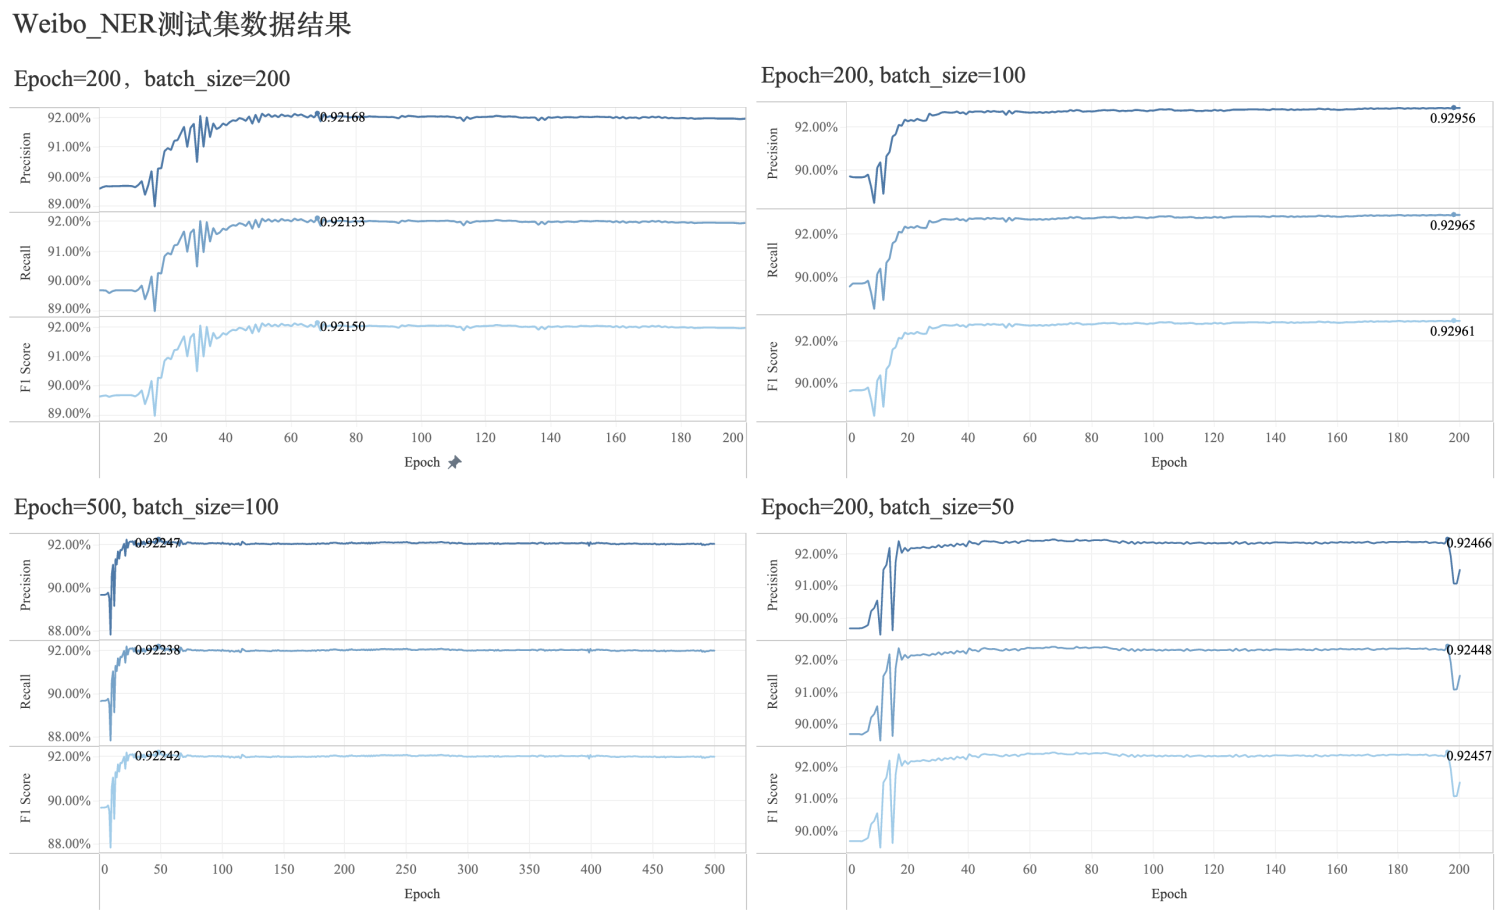
\includegraphics[width=14cm]{figures/weibo_ner_result.png}
    \caption{Weibo NER数据集测试结果}
\end{figure}

分别将epoch和batch\_size设置为(200, 200), (200, 100), (200, 50), (500, 100),Precision、Recall和F1 score随epoch变化
的趋势如图~\ref{fig:weibo_result}所示。可以看到Weibo数据集的字符级命名实体识别效果在(200, 100)的参数设置下F1值可以接近
93\%。


\subsubsection{MSRA数据集结果}

\begin{figure}[!htp]
    \centering
    \label{fig:MSRA_result}
    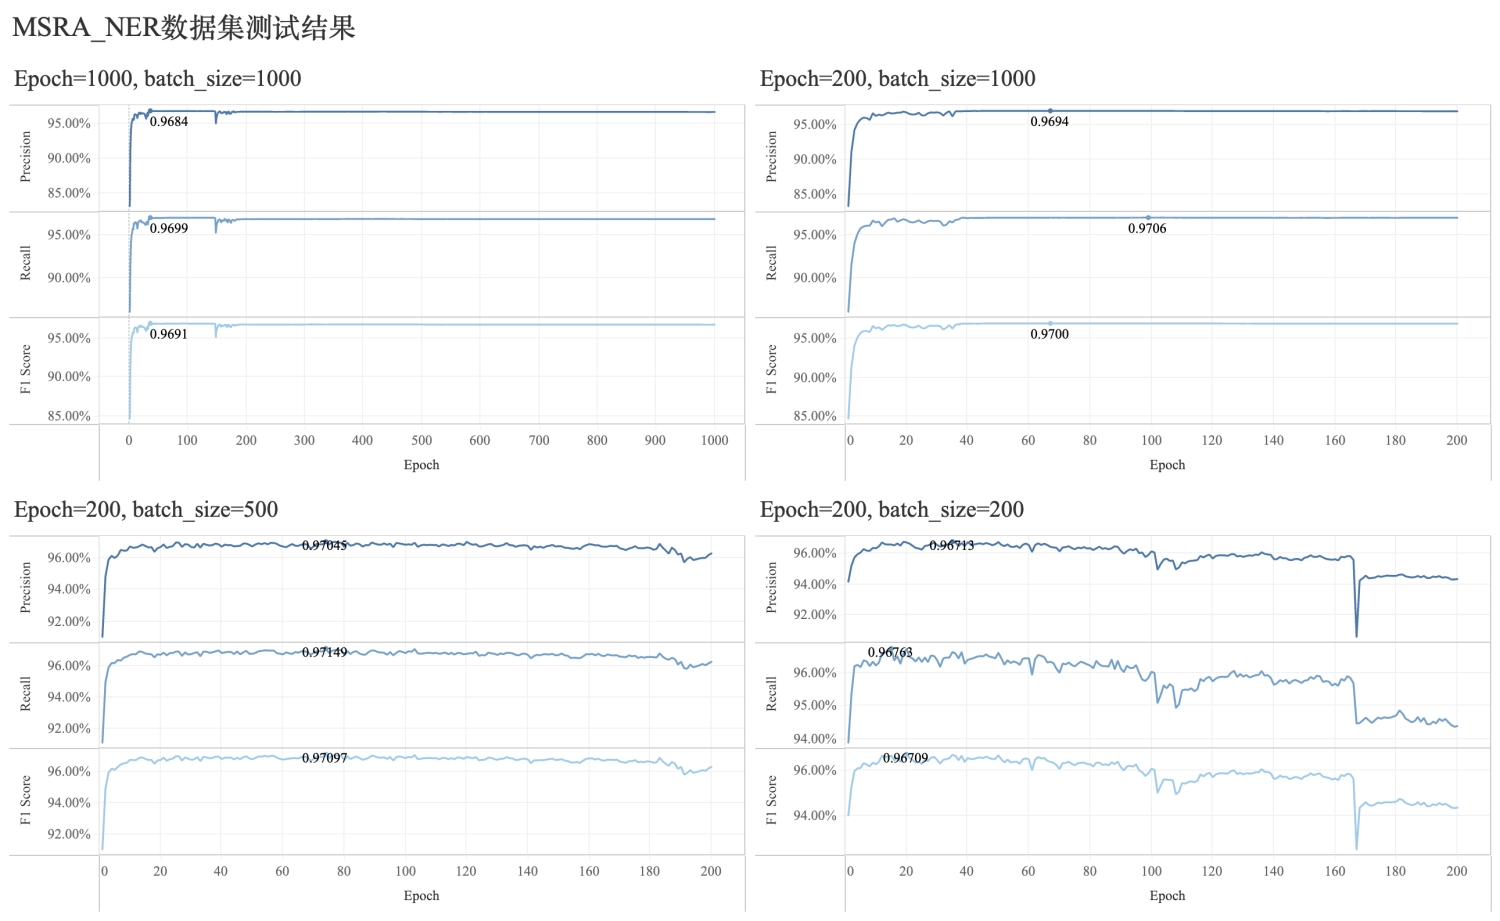
\includegraphics[width=14cm]{figures/MSRA_ner_result.png}
    \caption{MSRA数据集测试结果}
\end{figure}

分别将epoch和batch\_size设置为(1000, 1000)、(200, 1000)、(200, 500)、(200, 200),Precision、Recall和F1 score随epoch变化
的趋势如图~\ref{fig:MSRA_result}所示。可以看到MSRA数据集的字符级命名实体识别效果在(200, 500)的参数设置下F1值可以超过97\%。

% !TEX root = ../main.tex

\chapter{下一阶段研究计划}

\begin{itemize}
    \item \textbf{嵌入方式的优化}:使用粒度更细的嵌入方式表示文本信息。粗粒度的Embedding矩阵包含的信息量太少
    \item \textbf{论文阅读}:至少阅读10篇以上关于语言嵌入方面的论文,找到可以优化的地方
    \item \textbf{算法理论的对比分析补充}:为什么要用当前的算法,给出理论支撑
    \item \textbf{论文撰写}:重新梳理结构,理清story line。
\end{itemize}
% \input{contents/summary}

%TC:ignore

% 参考文献
\printbibliography[heading=bibintoc]

% 附录
% \appendix

% 附录中图表不加入索引
\captionsetup{list=no}

% % 附录内容
% \input{contents/app_maxwell_equations}
% \input{contents/app_flow_chart}

% 结尾部分
\backmatter

% 用于盲审的论文需隐去致谢、发表论文、科研成果、简历

% 致谢
% \input{contents/acknowledgements}

% 发表论文及科研成果
% 盲审论文中,发表论文及科研成果等仅以第几作者注明即可,不要出现作者或他人姓名
% \input{contents/achievements}

% 简历
% \input{contents/resume}

% 学士学位论文要求在最后有一个大摘要,单独编页码
% \input{contents/digest}

%TC:endignore

\end{document}
